\begin{slikaDesno}{fig/sc.pdf}
    {\color{red}*}\PID
    У колу са слике познато jе $C = C_{\rm s} = 100\unit{pF}$. 
    У почетном тренутку оба кондензатора су неоптерећена.
Прекидачи су идеални и затвараjу се наизменично,
краткотраjно, и то прво прекидач $\Uppi_1$ па прекидач
$\Uppi_2$. Напон генератора $v_{\rm U}$ не мења вредност осим када
jе прекидач $\Uppi_2$ затворен.
\end{slikaDesno}
\begin{enumerate}[label=(\alph*)]
    \item Одредити диференцну jедначину система чиjи jе
    jедини улаз напон побудног генератора $v_U[k]$ а jедини излаз напон 
    $v_{\rm I}[k]$ одређени након $k > 0$ затварања прекидача $\Uppi_1$.
    \item Одредити одзив добиjеног система на побуду $v_{\rm U}[k] = V_0 \uu[k]$ и 
    испитати његову асимптотску стабилност.
    \item[({\color{red}**}в)] Одредити отпорност отпорника $R$ који може да замени 
    структуру десно од кондензатора $C$ тако да се одбирци одскочног 
    одзива континуалног система одговарају добијеном дискретном одзиву у тренуцима 
    одабирања. У том случају, усвојити да се прекидачи затварају периодично, 
    учестаношћу $f$.
\end{enumerate}
\vspace*{2mm}

\textsc{\underline{Решење:}} Приликом затварања прекидача $\Uppi_2$ кондензатор $C_{\rm s}$ се врло брзо (практично тренутно) испразни, а 
приликом затварања прекидача $\Uppi_1$ у колу се деси проток наелектрисања, у грани са побудним генератором, који мења наелектрисање, односно напон, 
кондензатора $C$. Будући да се процес
наизменичног краткотрајног затварања прекидача $\Uppi_1$ па $\Uppi_2$ периодично понавља, тренутни напон тог кондензатора представља 
меморију овог система, што је описано дискретним сигналом $v_C = {v_C}[k]$. Када се прекидач затвори $k$-ти пут, напон генератора је 
$v_{\rm U} = v_{\rm U}[k]$. Непосредно пре тога, почетни напон кондензатора је $v_{C}[k-1] = v_{\rm U}[k-1] - v_{\rm I}[k-1]$, а
може се представити заменском шемом као што је приказано на слици \ref{\ID.zam_sch}. На основу те шеме, излазни напон ће бити 
одређен капацитивним раздеником, као
\begin{equation}
    v_{\rm I}[k] = \upalpha (v_{\rm U}[k] + v_{\rm I}[k-1] - v_{\rm U}[k-1] ),
\end{equation}
где је $\upalpha =  \dfrac{C}{C + C_{\rm s}}$ коефицијент капаицивног разденика напона.
Одавде се налази тражена диференцна једначина у облику 
\begin{equation}
    v_{\rm I}[k] - \upalpha v_{\rm I}[k-1] = \upalpha( v_{\rm U}[k] - v_{\rm U}[k-1] ) 
    \Leftrightarrow
    \underbrace{( 1 - \DD \upalpha )}_{P(\DD)} v_{\rm I}[k] = \underbrace{\upalpha(1 - \DD)}_{Q(\DD)} v_{\rm U}[k]
\end{equation}

(б) Израз са десне стране диференцне једначине може се поједноставити као 
$\underbrace{(1 - \DD)}_{Q(\DD)} v_{\rm U}[k] = \underbrace{\upalpha(1 - \DD)}_{Q(\DD)} V_0 \uu[k] =\upalpha V_0 \updelta[k]$, па је потребно 
решити диференцну једначину облика
\begin{equation}
    v_{\rm I}[k] - \upalpha v_{\rm I}[k-1] = \upalpha V_0 \updelta[k], \label{\ID.difeq}
\end{equation}
што се може учинити на сличан начин као у задатку \ref{z:diferencna_resi}. Карактеристични полином дате диференцне једначине је 
$P(\uplambda) = \uplambda - \upalpha$ чији је једини корен $\uplambda = \upalpha$ па је у овом случају једина карактеристична 
функција $\upalpha^k$,  односно је $v_{\rm I}[k] = A \upalpha^k \uu[k]$. Разматрајући израз \eqref{\ID.difeq} за $k=0$, усвајајући
да је $v_{\rm I}[k < 0] = 0$, има се $v_{\rm I}[0] = \upalpha V_0$, на основу чега мора бити коначно
\begin{equation}
    v_{\rm I}[k] = V_0 \upalpha^{k+1} \uu[k]. 
\end{equation}
За конкретно задате бројеве је $\upalpha = \dfrac{1}{2}$ па је временски дијаграм тог сигнала дат на слици 
\ref{\ID.fig.b}.

\begin{figure}
    \begin{subfigure}{0.49\textwidth}
        \centering
        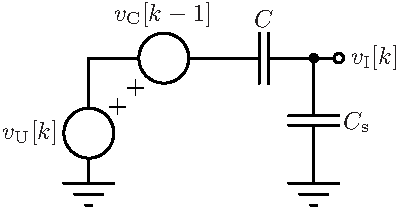
\includegraphics[scale=1]{fig/sc-sol.pdf}
        \caption{Са уведеном заменском шемом.}
        \label{\ID.zam_sch}
    \end{subfigure}
    %
    \begin{subfigure}{0.49\textwidth}
        \centering
        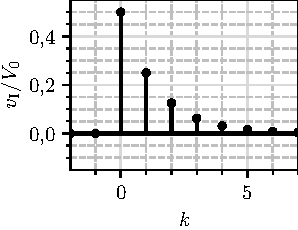
\includegraphics[scale=1]{fig/sc_plot.pdf}
        \caption{График дискретног излазног напона.}
        \label{\ID.fig.b}
    \end{subfigure}
\end{figure}

({\color{red}**}в) Треба да буде $R = \dfrac{1}{fC_{\rm s}}$.